% Made up for the tikra benchmark.
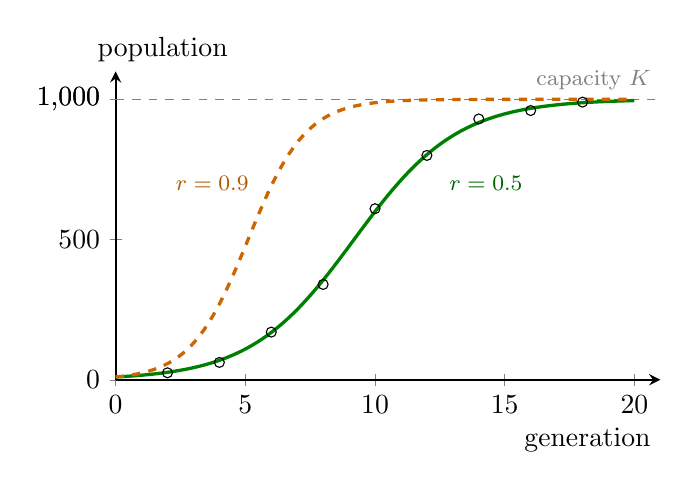
\begin{tikzpicture}
\begin{axis}[axis lines=left, axis line style={-stealth, thick},
    xmin=0, xmax=21, ymin=0, ymax=1100, width=8.5cm, height=5.5cm,
    xlabel={generation}, ylabel={population},
    ytick={0,500,1000}, extra y ticks={1000}, extra y tick style={grid=major,
      major grid style={dashed, gray}},
    every axis x label/.style={at={(axis description cs:1,0)}, anchor=north east, yshift=-14pt},
    every axis y label/.style={at={(axis description cs:0,1)}, anchor=south west, xshift=-10pt},
    domain=0:20, samples=100, clip=false]
  \addplot[very thick, green!50!black] {1000/(1+99*exp(-0.5*x))};
  \addplot[very thick, orange!80!black, dashed] {1000/(1+99*exp(-0.9*x))};
  \addplot[only marks, mark=o, mark size=1.8pt, black] coordinates {
    (2,25) (4,62) (6,170) (8,340) (10,610) (12,800) (14,930) (16,960) (18,990)};
  \node[font=\footnotesize, green!40!black, anchor=west] at (axis cs:12.5,700) {$r=0.5$};
  \node[font=\footnotesize, orange!70!black, anchor=east] at (axis cs:5.5,700) {$r=0.9$};
  \node[font=\footnotesize, gray, anchor=south east] at (axis cs:21,1000) {capacity $K$};
\end{axis}
\end{tikzpicture}
